\documentclass{article}
\usepackage{tikz}
\usetikzlibrary{shapes.geometric, arrows}

\tikzstyle{startstop} = [rectangle, rounded corners, minimum width=3cm, minimum height=1cm,text centered, draw=black, fill=red!30]
\tikzstyle{process} = [rectangle, minimum width=3cm, minimum height=1cm, text centered, draw=black, fill=orange!30]
\tikzstyle{decision} = [diamond, minimum width=3cm, minimum height=1cm, text centered, draw=black, fill=green!30]
\tikzstyle{arrow} = [thick,->,>=stealth]

\begin{document}

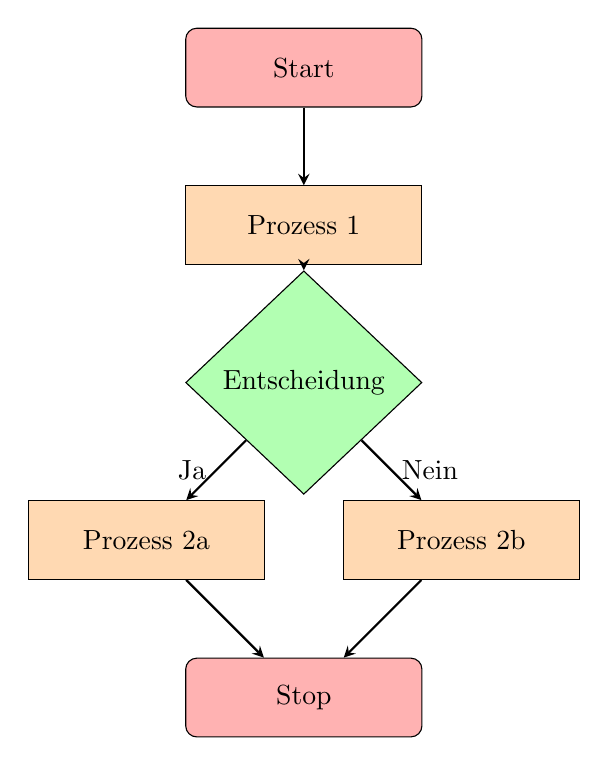
\begin{tikzpicture}[node distance=2cm]

\node (start) [startstop] {Start};
\node (pro1) [process, below of=start] {Prozess 1};
\node (dec1) [decision, below of=pro1] {Entscheidung};
\node (pro2a) [process, below of=dec1, xshift=-2cm] {Prozess 2a};
\node (pro2b) [process, below of=dec1, xshift=2cm] {Prozess 2b};
\node (stop) [startstop, below of=pro2a, xshift=2cm] {Stop};

\draw [arrow] (start) -- (pro1);
\draw [arrow] (pro1) -- (dec1);
\draw [arrow] (dec1) -- node[anchor=east] {Ja} (pro2a);
\draw [arrow] (dec1) -- node[anchor=west] {Nein} (pro2b);
\draw [arrow] (pro2a) -- (stop);
\draw [arrow] (pro2b) -- (stop);

\end{tikzpicture}

\end{document}